\begin{frame}{Алгоритм двухуровневой кластеризации}
    \begin{enumerate}
        \setcounter{enumi}{-1}
        \item
            Input: обычное BVH (DFS) \textbf{T} с размером указателей на дочерние узлы размером \textbf{n} бит
        \item
            Из корня дерева \textbf{T} создем адрессные кластеры \textbf{AC} \textit{по COLBVH}
        \item
            Для кадого дочернего \textbf{AC} создем \textit{glue node} \textbf{G}, "склеивая" с родительским узлом, 
            и повторяем \textbf{1}
        \item
            Для каждого \textbf{AC} мы рекурсивно создаем кэш-кластеры \textbf{CC} \textit{по COLBVH}
    \end{enumerate}
    \begin{figure}
        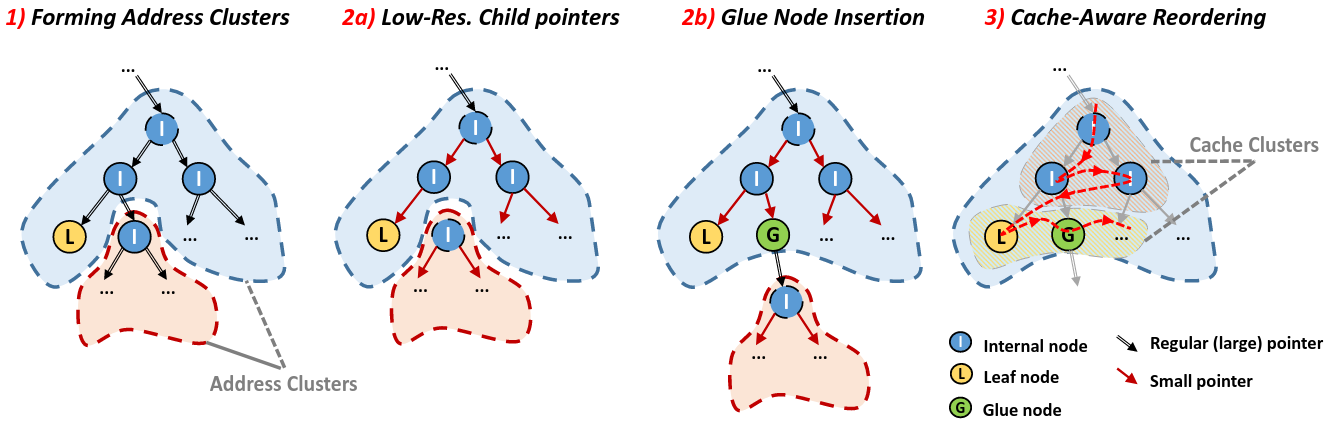
\includegraphics[keepaspectratio, width=\textwidth]{res/2lvl_clustering.png}
    \end{figure}
\end{frame}

\begin{frame}[fragile]{Кластеры адресов. Функция BuildAC}
    \framesubtitle{Двухуровневая кластеризация}
    \begin{lstlisting}[language=C++,basicstyle=\ttfamily,keywordstyle=\color{blue}]
BuildAC(dstOffset, srcRoot) -> offset_t
    maxN = 2^ptr_bits; AC = {}
    child_nodes = {src_root}; child_ACs = {}
    while ((size(AC + children) < maxN)
        && !children.is_empty)
        node = pop_max_SA(child_nodes)
        AC << node
        if (is_internal(node))
            children << node.left << node.right
    for (node : child_nodes)
        if (is_internal(node))
            child_ASs << node << make_glue(node)
        else
            AC << node
    ...
    \end{lstlisting}
\end{frame}

\begin{frame}[fragile]{Кластеры адресов. Функция BuildAC (продолжение)}
    \framesubtitle{Двухуровневая кластеризация}
    \begin{lstlisting}[language=C++,basicstyle=\ttfamily,keywordstyle=\color{blue}]
dst_offset += BUILDCCS(dst_offset, AC)
for (root_node : roots(child_ACs))
    dst_offset = align(dst_offset, cache_layout)
    update_parent_glue_node(root_node)
    dst_offset = BuildAC(dst_offset, root_node)
return dst_offset
    \end{lstlisting}
    \begin{block}{update\_parent\_glue\_node()}
        Офсеты корней дочерних кластеров неизвестны на момент создания склеивающего узла,
        а значит должны быть занесены в \textit{glue nodes} позже
    \end{block}
    \begin{block}{}
        Чтобы шаг кэш-кластеринга имел смысл, нужно чтобы корень каждого \textbf{AC} был
        выровнен по размеру кэш-линии
    \end{block}
\end{frame}

\begin{frame}[fragile]{Кэш-кластеры. Функция BuildCCs}
    \framesubtitle{Двухуровневая кластеризация}
    \begin{adjustbox}{width=\textwidth, keepaspectratio}
        \begin{lstlisting}[language=C++,basicstyle=\ttfamily,keywordstyle=\color{blue}]
BuildCCs(dst_offset, AC) -> offset_t
    maxN = cache_line_size / node_size
    CC_roots = get_root(AC); deferred_CCs = {}
    while (!CC_roots.is_empty)
        child_nodes << CCRoots; CC = {}
        while (size(CC) < maxN && !child_nodes.empty)
            node = pop_max_SA(child_nodes)
            CC << node
            if (is_internal(node))
                childNodes << node.left << node.right
        CC_roots << {childNodes + CCRoots} // DFS
        if (size(CC) == maxN)
            dst_offset = WriteCluster(dst_offset, CC)
        else deferred_CCs << CC
    for (CC : deferred_CCs) // complete but not full
        dst_offset = WriteCluster(dst_offset, CC)
    return dst_offset
    \end{lstlisting}
\end{adjustbox}
\end{frame}

\begin{frame}[fragile]{Кэш-кластеры. Функция WriteCluster}
    \framesubtitle{Двухуровневая кластеризация}
    \begin{block}{}
        Функция \textit{WriteCluster} записывает кэш-кластер в \textbf{BVH}
    \end{block}
    \begin{lstlisting}[language=C++,basicstyle=\ttfamily,keywordstyle=\color{blue}]
WriteCluster(dst_offset, CC) -> offset_t
    update_child_ptr(get_parent(CC[0]));
    for (i in [0; size(CC)])
        dstBVH[dst_offset] = CC[i];
        dst_offset++
    return dst_offset
    \end{lstlisting}
    \begin{block}{update\_child\_ptr()}
        Записать указатели на дочерние узлы, адресс которых мы не знали раньше
    \end{block}
\end{frame}

\begin{frame}[t]{Дальнейшие оптимизации}
    \framesubtitle{Двухуровневая кластеризация}
    \begin{itemize}
        \item
            \textbf{Padding}:
            Кэш-кластер, следующий за неплолным кэш-кластером, стоит хранить с отступом от него -
            так, чтобы начало \textbf{CC} совпадало с началом кэш-линии

            \textit{Нужно следить (ограничивать паддинг), чтобы узлы не выходили за пределы \textit{small pointers}}
        \item
            \textbf{Cluster merging}:
            Можно объединять малетьнькие собранные кластеры, объединяя их узлы и сортируя по SA.
            Чтобы более большие узлы были загружены в кэш-линию
    \end{itemize}
\end{frame}

\begin{frame}[t]{Структура узла}
    \framesubtitle{Двухуровневая кластеризация}
    Для имплементации двухуровневой кластеризации было необходимо уменьшить размер узла:
    \begin{itemize}
        \item
            \textbf{Сокращение информации}: \textit{повторное использование плоскостей родительских узлов}

            Для пары дочерних узлов храним 6 плоскостей и \textit{reuse mask}
        \item
            \textbf{Снижение точности}: \textit{квантизация узла}

            Кол-во квантизированных битов определяет компромисс между объемом памяти и качеством BVH

    \end{itemize}

    \begin{figure}
        \begin{center}
            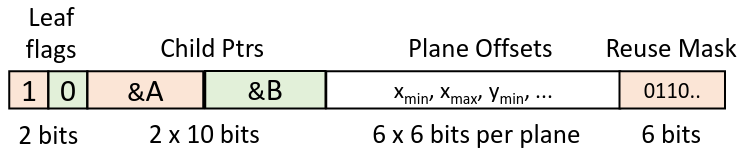
\includegraphics[keepaspectratio, width=\textwidth]{res/8byte_node.png}
        \end{center}
    \end{figure}
\end{frame}

\begin{frame}{Аппаратная поддержка. Traversal cluster}
    \framesubtitle{Двухуровневая кластеризация}
    Pipelined and multi-threaded units for out-of-order processing:
    \begin{columns}
        \column{0.5\textwidth}
        \begin{itemize}
            \item 
                \textbf{Traversal Unit (TU)}
                Делает обход 1 ray/tread и хранит его состояние.
                \begin{itemize}
                    \item 
                        распаковывает BB
                    \item 
                        вычисляет \textit{ray-BB} пересечения
                    \item 
                        обновляет стек для треда
                \end{itemize}
            \item 
                \textbf{Leaf Unit (LU)}
                Исходя из флагов
                \textit{(glue node/primitives)}:
                \begin{itemize}
                    \item 
                        \textit{передает луч в \textit{PU}}
                    \item 
                        \textit{возвращает адресс для \textit{TU} из glue node}
                \end{itemize}
        \end{itemize}
        \column{0.5\textwidth}
        \begin{figure}
            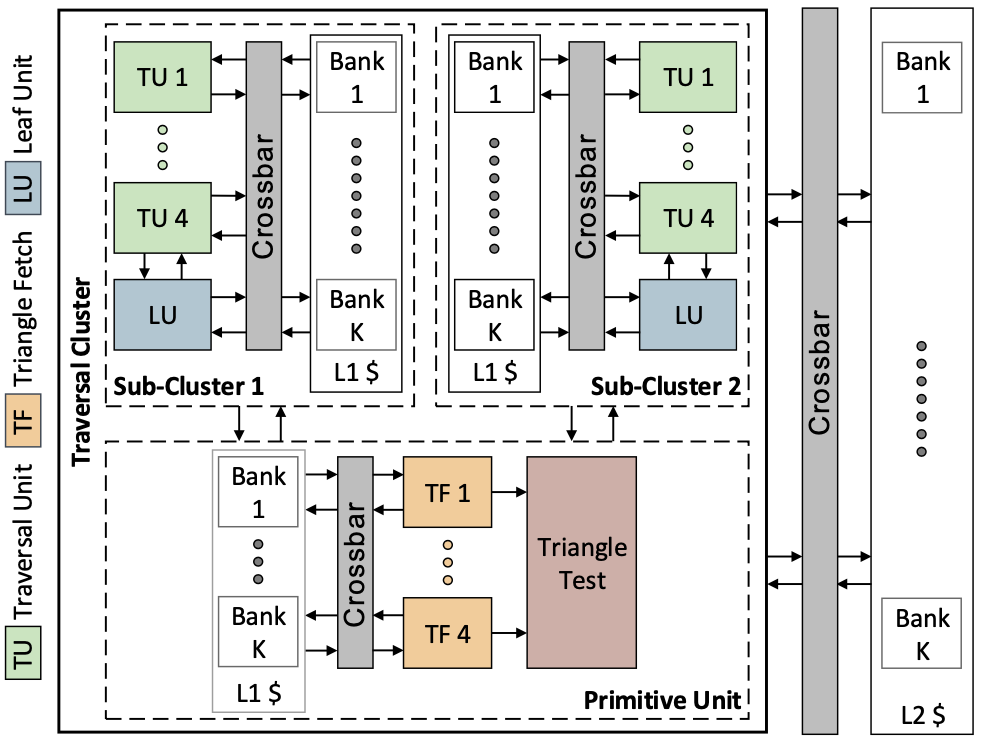
\includegraphics[keepaspectratio,
            width=\textwidth]{res/block_diagram.png}
        \end{figure}

        \begin{itemize}
            \item 
                \textbf{Primitive Unit (PU)}
                Возвращает результаты тестов пересечения с треугольниками в \textbf{TU}
        \end{itemize}

    \end{columns}

\end{frame}

\begin{frame}[t]{Плюсы и минусы}
    \framesubtitle{Двухуровневая кластеризация}
    \textbf{Достоинства}
    \begin{itemize}
        \item
            уменьшение \textit{cache misses}
        \item
            уменьшение кол-ва подгружаемой в кэш памяти
        \item
            сжатое представление узлов
        \item
            универсальность подхода (ничто не мешает изменить
            способ кластерирования и способ записи узлов)
    \end{itemize}
    \textbf{Недостатки}
    \begin{itemize}
        \item
            время построения BVH неоптимизированно
    \end{itemize}
\end{frame}

